\documentclass{article}
%\usepackage[spanish,activeacute]{babel}
%\usepackage[english,activeacute]{babel}
%\usepackage[latin1]{inputenc}
\usepackage[utf8]{inputenc}
\usepackage[english]{babel}

\usepackage{amsmath,amsfonts,amssymb,amstext,amsthm,amscd}
\usepackage{hyperref}
\usepackage{latexsym}
\usepackage{graphicx}
%\usepackage{subfigure}
\usepackage{subfig}
%\linespread{1.6}
\usepackage{float}
\usepackage{dcolumn}% Align table columns on decimal point(esto lo saque del ejemplo de revtex4)
\usepackage{bm}% bold math(esto lo saque del ejemplo de revtex4)
\newcounter{itemR}
\usepackage{here} %recordar usar el comando[H] para las gráficas que es el comando here en lugar de [h!]
\usepackage{fancyhdr}
%\usepackage{sidecap}
%\usepackage[spanish,activeacute]{babel}
\usepackage{multirow}
\usepackage{multicol}
\usepackage{array}
\usepackage{enumitem}
%\usepackage{booktabs}% para hacer tablas profesionales con \toprule

% ------------------------------------------------------------------------------------------------------------------------------------------------------

\usepackage{fancyhdr}
\setlength{\headheight}{15.2pt}
\usepackage[paperwidth=8.5in, paperheight=11.0in, top=1.0in, bottom=1.0in, left=1.0in, right=1.0in]{geometry}

\pagestyle{fancyplain}
\fancyhead[LE,RO]{Práctica $\#$6}
\fancyhead[CE,CO]{}
\fancyhead[RE,LO]{P23-FIS1012-12}
\fancyfoot[LE,RO]{\thepage}
\fancyfoot[CE,CO]{Laboratorio de Física, UDLAP}
\fancyfoot[RE,LO]{}

% ------------------------------------------------------------------------------------------------------------------------------------------------------
% ------------------------------------------------------------------------------------------------------------------------------------------------------
% ------------------------------------------------------------------------------------------------------------------------------------------------------

\begin{document}

\fancypagestyle{plain}{
   	\renewcommand{\headrulewidth}{1pt}
   	\renewcommand{\footrulewidth}{1pt}
}

\renewcommand{\footrulewidth}{1pt}
\renewcommand{\tablename}{Tabla}
\renewcommand{\figurename}{Figura}

% ------------------------------------------------------------------------------------------------------------------------------------------------------
% ------------------------------------------------------------------------------------------------------------------------------------------------------
% ------------------------------------------------------------------------------------------------------------------------------------------------------

\title{Resistencia}
\author{\small{Luis Alberto Gil Bocanegra ID: 177410, Erick Gonzalez Parada ID: 178145}\\
 \small{Gartzen Aldecoa Barroso ID: 178034 .}\\		% ----- Varios autores separarlos por comas:  \small{Nombre(s) de (los) autor(es)\footnote{ID; correo@udlap.mx}, Nombre(s) de (los) autor(es)\footnote{ID; correo@udlap.mx}
	   \small{Depto. de Actuaría, Física y Matemáticas, Universidad de las Américas Puebla, Puebla, M\'exico 72810}}
\date{\small{\today}}

\maketitle

% ------------------------------------------------------------------------------------------------------------------------------------------------------
% ------------------------------------------------------------------------------------------------------------------------------------------------------
% ------------------------------------------------------------------------------------------------------------------------------------------------------

\begin{abstract}
	Esta práctica se hicieron dos partes, en la primera se determino la resistencia de 3 alambres 
	midiendo el material cada 10 cm para sacar la resistencia de cada pedazo y ver si kappa coincide con el material.
	Para la segunda parte se gráfico también la resistencia con respecto a la temperatura y como cambiaba.
\\
\\
{\it Keywords:}  resistencia, kappa
\\
\\
\end{abstract}

% ------------------------------------------------------------------------------------------------------------------------------------------------------

\begin{multicols}{2}
\section{Desarrollo teórico}\label{Desarrollo Teorico}                              	% -------------------- Introducción
\cite{Fluke}
En la física, la resistencia eléctrica es una propiedad fundamental de los materiales que se opone al flujo de corriente eléctrica. En esta sección, exploraremos las expresiones relacionadas con la resistencia eléctrica.

\subsection{Corriente en un Punto ($\mathbf{i}$)}

La corriente en un punto ($\mathbf{i}$) se define como la tasa de cambio de carga con respecto al tiempo y se expresa como:

\begin{equation}
    \mathbf{i} = \frac{d\mathbf{q}}{dt}
\end{equation}

donde:
$\mathbf{i}$ es la corriente en un punto,
$d\mathbf{q}$ es el cambio infinitesimal de carga en un elemento de volumen,
$dt$ es el cambio infinitesimal de tiempo.

\subsection{Relación entre Densidad de Corriente y Corriente Total}

La corriente eléctrica total ($i$) a través de un conductor se obtiene integrando la densidad de corriente ($\mathbf{J}$) sobre el área transversal ($A$) del conductor:

\begin{equation}
    i = \int \mathbf{J} \cdot d\mathbf{A}
\end{equation}

donde:
$i$ es la corriente total,
$\mathbf{J}$ es la densidad de corriente,
$d\mathbf{A}$ es el elemento infinitesimal de área sobre la sección transversal.

\subsection{Relación entre Corriente, Área y Densidad de Corriente}

La densidad de corriente ($\mathbf{J}$) está relacionada con la corriente total ($i$) y el área transversal ($A$) del conductor mediante la expresión:

\begin{equation}
    \mathbf{J} = \frac{i}{A}
\end{equation}

donde:
$\mathbf{J}$ es la densidad de corriente,
$i$ es la corriente total,
$A$ es el área transversal del conductor.

\subsection{Ley de Ohm}

La relación fundamental entre la diferencia de potencial ($\Delta V$), la corriente ($i$) y la resistencia eléctrica ($R$) en un circuito se expresa mediante la Ley de Ohm:

\begin{equation}
    \Delta V = i \cdot R
\end{equation}

donde:
$\Delta V$ es la diferencia de potencial (voltaje),
$i$ es la corriente,
$R$ es la resistencia eléctrica.

La resistencia eléctrica ($R$) se define como la proporción entre la diferencia de potencial ($\Delta V$) y la corriente ($i$).
\section{Desarrollo Experimental}\label{Desarrollo experimental}				% -------------------- Metodología 
\subsection*{Lista de Materiales}
A continuación se presenta una lista de materiales:
\subsection*{parte 1}
\begin{enumerate}
    \item Tabla de resistencia variable
    \item Multímetro
    \item Vernier digital
\end{enumerate}
\subsection*{parte 2}
\begin{enumerate}
    \item horno eléctrico
    \item Multímetro
    \item Sonda tipo k
    \item Placa de cerámica
    \item Resistencias en cerámica
\end{enumerate}

Para la primera parte se tenían los 3 alambres uno de cobre, otro de níquel y latón con el vernier
se mide cada 10 cm la resistencia que se captura con el multímetro y se gráfico resistencia x longitud y se calculo 
el área y con ello la resistividad. 
\\
 Para la segunda parte teníamos un alambre en donde con la placa de cerámica montada para poner el horno colocamos 
 el alambre de tal manera que quede "atravesado" con el horno y podamos medir la diferencia de la resistencia con respecto al cambio de temperatura.
 \end{multicols}
\section{Resultados y análisis}\label{Resultados}			% -------------------- Resultados
\subsection*{parte 1}
\begin{table}[H]
    \centering
    \begin{tabular}{|c|c|c|c|}
    \hline
    Alambre material & Diámetro & Área & Resistividad \\
    \hline
    cobre & 0.0062 mm & 0.01947792 & 0.017619726 \\
    latón & 0.006 mm & 0.0188496 & 0.018302962 \\
    cromo-níquel & 0.0072 mm & 0.02261952 & 0.022492851 \\
    \hline
    \end{tabular}
    \caption{Valores de Material, Diámetro, Área y Resistividad}
    \label{tabla:1}
\end{table}

\begin{figure}[H]
	\centering
	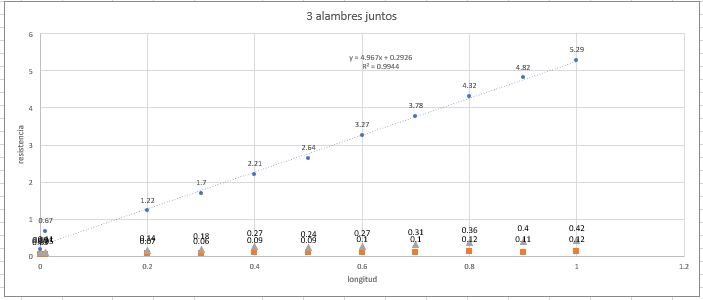
\includegraphics[scale=0.6]{../imgs/al.png}
	\caption{Resistencia vs longitud}
	\label{fig:1}
\end{figure}

\subsection*{parte 2}

\begin{figure}[H]
	\centering	
	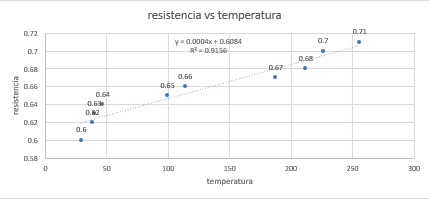
\includegraphics[scale=0.5]{../imgs/tem.png}
	\caption{Resistencia vs temperatura}
	\label{fig:2}
\end{figure}

\begin{table}[ht]
    \centering
    \begin{tabular}{|c|c|}
    \hline
    Parámetro de T & Comparativa \\
    \hline
    0.017833984 & Cobre \\
    \hline
    0.017258694 & Cobre \\
    \hline
    0.020710433 & Aluminio \\
    \hline
    \end{tabular}
    \caption{Comparativa de Parámetros}
    \label{tabla:comparativa}
\end{table}


\section{Conclusiones}\label{Conclusiones}				% -------------------- Conclusiones
Como equipo concluimos que el objetivo no se cumplió del todo ya que nos vario bastante kappa con respecto a cualquier tabla donde muestra la kappa de cada material
y esto puede ser provocado por la falta de calibración en los sistemas que nos dan para medir las variables. 
\\
Con respecto al objetivo de la segunda parte en esta si se cumplió ya que el objetivo de eso era identificar el cambio, y en ese caso fue lo primero que se identifico 
al realizar esa parte del experimento.
\begin{thebibliography}{9}						% -------------------- Bibliografía
	\bibitem{Fluke}
	Fluke. (s. f.). ¿Qué es la resistencia? Fluke. https://www.fluke.com/es-mx/informacion/blog/electrica/que-es-la-resistencia
	\bibitem{Serway}
	Serway, R. A., $\&$ Jewett, J. W. (2008). Física para ciencias e ingeniería. (7.a
ed., Vol. 1). CENGAGE Learning.

\bibitem{Pérez}
	Newton, I. (1687). Philosophiæ Naturalis Principia Mathematica [Mathematical Principles of Natural Philosophy]. Londini: Jussu Societatis Regiæ ac Typis Josephi Streater.

\end{thebibliography}
\end{document}	